% !TeX program = xelatex
\documentclass[aspectratio=169]{beamer}

% Theme selection
\usetheme{metropolis}

% Packages
\usepackage{fontspec}
\usepackage{xcolor}
\usepackage{listings}
\usepackage{sourcecodepro} % Use Source Code Pro for monospaced text if available
\usepackage{tikz}
\usetikzlibrary{positioning}

% Color Palette - "Hacky" / Cyberpunk / Terminal
\definecolor{bgdata}{HTML}{1a1a1a} % Dark background
\definecolor{fgdata}{HTML}{00ff00} % Neon Green text
\definecolor{accent}{HTML}{ff00ff} % Neon Pink accent
\definecolor{comment}{HTML}{6272a4} % Muted blue/purple for comments
\definecolor{keyword}{HTML}{ff79c6} % Pink for keywords
\definecolor{string}{HTML}{f1fa8c} % Yellow for strings

% Apply Colors
\setbeamercolor{background canvas}{bg=bgdata}
\setbeamercolor{normal text}{fg=white} % Keep main text readable (white), use green for highlights
\setbeamercolor{frametitle}{bg=bgdata, fg=fgdata}
\setbeamercolor{title}{fg=fgdata}
\setbeamercolor{subtitle}{fg=accent}
\setbeamercolor{structure}{fg=accent} % Itemize bullets, etc.
\setbeamercolor{alerted text}{fg=accent}

% Font Customization (Try to simulate a terminal feel)
\setsansfont{FiraCode}[
    Path = /usr/share/fonts/TTF/,
    Extension = .ttf,
    UprightFont = *-Regular,
    BoldFont = *-Bold
]
\setmonofont{FiraCode}[
    Path = /usr/share/fonts/TTF/,
    Extension = .ttf,
    UprightFont = *-Regular,
    BoldFont = *-Bold
]

% Code Listing Style
\lstset{
    basicstyle=\ttfamily\small\color{white},
    keywordstyle=\color{keyword}\bfseries,
    commentstyle=\color{comment}\itshape,
    stringstyle=\color{string},
    backgroundcolor=\color{bgdata},
    frame=single,
    rulecolor=\color{fgdata}, % Green frame
    breaklines=true,
    numbers=left,
    numberstyle=\tiny\color{comment},
    captionpos=b,
    tabsize=2
}

% Beamer Template Tweaks
\setbeamertemplate{frame numbering}[fraction]
\setbeamertemplate{navigation symbols}{} % Remove navigation symbols

% Title Info
\title{Reussir}
\subtitle{A Memory Reuse IR Playground for FP Languages}
\author{Schrodinger Zhu} % Assuming user name based on context
\date{\today}

\begin{document}

\begin{frame}
    \titlepage
\end{frame}

\begin{frame}{Overview}
    \tableofcontents
\end{frame}

\section{Introduction}

\begin{frame}{Foundations}
    \begin{quote}
        ``\dots This suggests an answer to our original question, at least within the framework of interaction nets: the fundamental laws of computation are \alert{commutation} and \alert{annihilation}.''
    \end{quote}
    \vspace{1em}
    \hfill --- Yves Lafont, \textit{Interaction Combinators}, 1997.
\end{frame}

\begin{frame}{The FP Connection}
    \begin{itemize}
        \item \textbf{Annihilation} $\leftrightarrow$ \alert{Elimination} (Pattern Matching / Destructors)
        \item \textbf{Commutation} $\leftrightarrow$ \alert{Introduction} (Constructors / Structural rules)
    \end{itemize}
    \vspace{1em}
    Functional programs are built from Intro/Elim pairs --- each pair is
    a potential \alert{memory reuse} opportunity.
    \texttt{Reussir} makes these interactions explicit at the IR level.
\end{frame}

\section{Examples}

\begin{frame}[fragile]{List Reversal}
    \begin{lstlisting}[language=Haskell, basicstyle=\ttfamily\small\color{white}]
enum List<T> { Nil, Cons(T, List<T>) }

fn reverse_impl(list : List<i32>, acc : List<i32>) -> List<i32> {
    match list {
        List::Nil => acc,
        List::Cons(x, xs) => reverse_impl(xs, List::Cons{x, acc})
    }
}

pub fn reverse(list : List<i32>) -> List<i32> {
    reverse_impl(list, List::Nil)
}
    \end{lstlisting}
    \small \texttt{Cons(x, xs)} is eliminated; a new \texttt{Cons\{x, acc\}} is introduced
    --- the eliminated cell can be \alert{reused in-place} for the introduction.
\end{frame}

\begin{frame}[fragile]{RBTree: Balancing (1/2)}
    \begin{lstlisting}[language=Haskell, basicstyle=\ttfamily\scriptsize\color{white}]
enum [value] Color { Red, Black }
enum Tree<T : Num> {
    Branch(Color, Tree<T>, T, Tree<T>),
    Leaf
}

fn balance_left<T : Num>(l : Tree<T>, k : T, r : Tree<T>) -> Tree<T> {
    match l {
        Tree::Branch(_, Tree::Branch(Color::Red, lx, kx, rx), ky, ry) =>
            Tree::Branch{
                Color::Red,
                Tree::Branch{Color::Black, lx, kx, rx},
                ky,
                Tree::Branch{Color::Black, ry, k, r}
            },
        // ... (continued)
    \end{lstlisting}
\end{frame}

\begin{frame}[fragile]{RBTree: Balancing (2/2)}
    \begin{lstlisting}[language=Haskell, basicstyle=\ttfamily\scriptsize\color{white}]
        // ... (continued)
        Tree::Branch(_, ly, ky, Tree::Branch(Color::Red, lx, kx, rx)) =>
            Tree::Branch{
                Color::Red,
                Tree::Branch{Color::Black, ly, ky, lx},
                kx,
                Tree::Branch{Color::Black, rx, k, r}
            },

        Tree::Branch(_, lx, kx, rx) =>
            Tree::Branch{
                Color::Black,
                Tree::Branch{Color::Red, lx, kx, rx},
                k,
                r
            },

        Tree::Leaf => Tree::Leaf
    }
}
    \end{lstlisting}
\end{frame}

\section{Background}

\begin{frame}{The Cost of Abstraction}
    FP relies heavily on heap-allocated objects.
    \alert{Memory management} is both essential and expensive.
    \begin{itemize}
        \item \textbf{Haskell, OCaml}: sophisticated Garbage Collectors (GC).
        \item \alert{Tradeoffs}: Latency, pauses, memory overhead.
    \end{itemize}
\end{frame}

\begin{frame}{Evolving Solutions}
    Languages are evolving to mitigate GC costs:
    \begin{itemize}
        \item \textbf{Haskell}: Introduced \alert{Linear Types} for resource control.
        \item \textbf{OCaml (Jane Street)}: Exploring \alert{local/stack allocation} strategies.
    \end{itemize}
\end{frame}

\begin{frame}{The RC Alternative}
    \textbf{Lean4} and \textbf{Koka} adopt a different approach:
    \begin{itemize}
        \item Reference Counting (RC) system.
        \item \alert{Functional-But-In-Place (FBIP)}:
        \begin{itemize}
            \item If an object has $\texttt{RC}=1$ (exclusive ownership), mutate it in place!
            \item Enables efficient mutation within functional purity.
        \end{itemize}
    \end{itemize}
    \vspace{0.5em}
    \textbf{Thesis}: FBIP has \alert{more potential} than prior work reveals.
\end{frame}

\section{Reussir's Design}

\begin{frame}{What We Present}
    FBIP has \alert{more potential} than existing work reveals.
    \vspace{0.5em}
    \begin{enumerate}
        \item \textbf{Structured Control Flow} --- generalize FBIP reuse beyond
              pattern matching to loops, branches, early returns
              (analogous to MLIR's bufferization).
        \item \textbf{Codegen Impact} --- case study on how token reuse and
              inc/dec cancellation improve generated code quality
              (not emphasized in prior work).
        \item \textbf{Lightweight FFI} --- RC-based runtime embeds an ownership
              model into the imperative world (\texttt{repr(C)} headers,
              polymorphic FFI templates).
        \item \textbf{Mixed Memory Management} --- combine RC with region-based
              allocation for local mutable objects (flex $\to$ freeze $\to$ rigid).
    \end{enumerate}
\end{frame}

\begin{frame}{Overall Design}
    \centering
    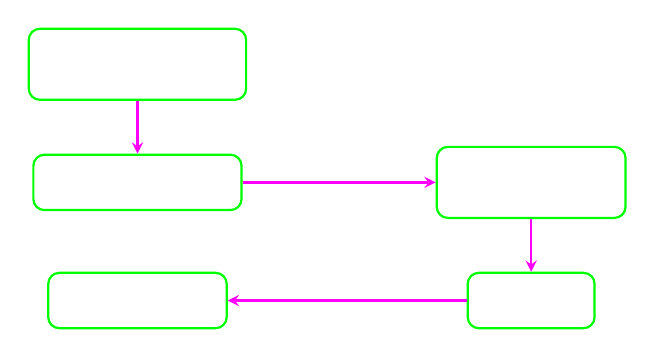
\begin{tikzpicture}[
        node distance=1.5cm,
        every node/.style={
            rectangle, 
            draw=fgdata, 
            thick, 
            text=white,
            align=center,
            rounded corners,
            minimum height=2em,
            font=\small
        },
        arrow/.style={
            ->, 
            >=stealth, 
            thick, 
            color=accent
        }
    ]
        \node (src) {Rust-alike Syntax\\FP Program};
        \node (front) [below of=src] {Haskell Frontend};
        \node (mlir) [right of=front, node distance=5cm] {MLIR Backend\\Optimization};
        \node (llvm) [below of=mlir] {LLVM IR};
        \node (bin) [left of=llvm, node distance=5cm] {Machine Code};

        \draw[arrow] (src) -- (front);
        \draw[arrow] (front) -- (mlir);
        \draw[arrow] (mlir) -- (llvm);
        \draw[arrow] (llvm) -- (bin);
    \end{tikzpicture}
\end{frame}

\begin{frame}{MLIR Backend Optimization}
    \centering
    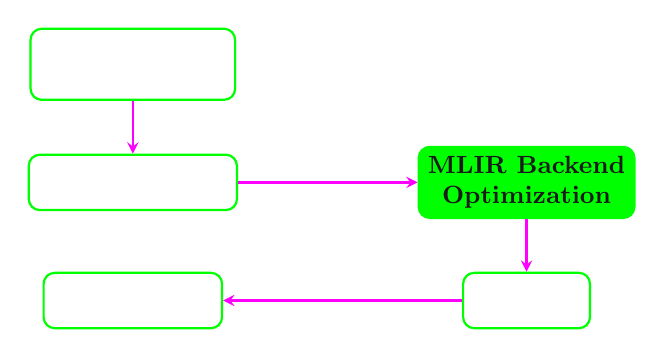
\begin{tikzpicture}[
        node distance=1.5cm,
        every node/.style={
            rectangle, 
            draw=fgdata, 
            thick, 
            text=white,
            align=center,
            rounded corners,
            minimum height=2em,
            font=\small
        },
        arrow/.style={
            ->, 
            >=stealth, 
            thick, 
            color=accent
        },
        highlight/.style={
            fill=fgdata,
            text=bgdata,
            font=\small\bfseries
        }
    ]
        \node (src) {Rust-like Syntax\\FP Program};
        \node (front) [below of=src] {Haskell Frontend};
        \node (mlir) [right of=front, node distance=5cm, highlight] {MLIR Backend\\Optimization};
        \node (llvm) [below of=mlir] {LLVM IR};
        \node (bin) [left of=llvm, node distance=5cm] {Machine Code};

        \draw[arrow] (src) -- (front);
        \draw[arrow] (front) -- (mlir);
        \draw[arrow] (mlir) -- (llvm);
        \draw[arrow] (llvm) -- (bin);
    \end{tikzpicture}
\end{frame}


\section{Compilation Pipeline}

\begin{frame}[fragile]{Detailed Compilation Pipeline}
    \centering
    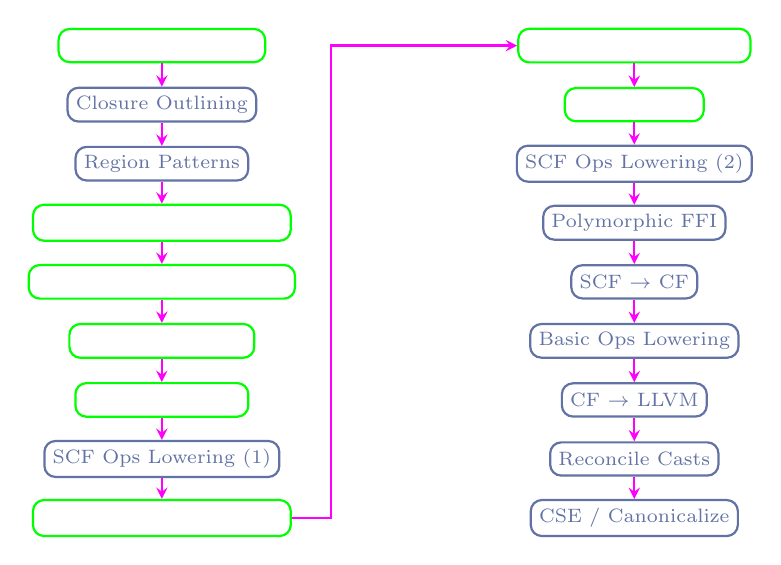
\begin{tikzpicture}[
        node distance=0.75cm,
        every node/.style={
            rectangle, 
            draw=fgdata, 
            thick, 
            text=white,
            align=center,
            rounded corners,
            font=\scriptsize,
            minimum height=1.2em,
            inner sep=3pt,
            anchor=center
        },
        dimmed/.style={
            draw=comment,
            text=comment
        },
        arrow/.style={
            ->, 
            >=stealth, 
            thick, 
            color=accent
        }
    ]
        % Column 1
        \node (p1) {Token Instantiation};
        \node (p2) [below of=p1, dimmed] {Closure Outlining};
        \node (p3) [below of=p2, dimmed] {Region Patterns};
        \node (p4) [below of=p3] {Inc/Dec Cancellation (1)};
        \node (p5) [below of=p4] {RC Decrement Expansion};
        \node (p6) [below of=p5] {Infer Variant Tag};
        \node (p7) [below of=p6] {Drop Expansion};
        \node (p8) [below of=p7, dimmed] {SCF Ops Lowering (1)};
        \node (p9) [below of=p8] {Inc/Dec Cancellation (2)};

        % Column 2
        \node (p10) [right of=p1, node distance=6cm] {Drop Logic Expansion};
        \node (p11) [below of=p10] {Token Reuse};
        \node (p12) [below of=p11, dimmed] {SCF Ops Lowering (2)};
        \node (p13) [below of=p12, dimmed] {Polymorphic FFI};
        \node (p14) [below of=p13, dimmed] {SCF $\to$ CF};
        \node (p15) [below of=p14, dimmed] {Basic Ops Lowering};
        \node (p16) [below of=p15, dimmed] {CF $\to$ LLVM};
        \node (p17) [below of=p16, dimmed] {Reconcile Casts};
        \node (p18) [below of=p17, dimmed] {CSE / Canonicalize};

        % Edges Col 1
        \draw[arrow] (p1) -- (p2);
        \draw[arrow] (p2) -- (p3);
        \draw[arrow] (p3) -- (p4);
        \draw[arrow] (p4) -- (p5);
        \draw[arrow] (p5) -- (p6);
        \draw[arrow] (p6) -- (p7);
        \draw[arrow] (p7) -- (p8);
        \draw[arrow] (p8) -- (p9);

        % Connection Col 1 -> Col 2
        \draw[arrow] (p9.east) -- ++(0.5,0) |- (p10.west);

        % Edges Col 2
        \draw[arrow] (p10) -- (p11);
        \draw[arrow] (p11) -- (p12);
        \draw[arrow] (p12) -- (p13);
        \draw[arrow] (p13) -- (p14);
        \draw[arrow] (p14) -- (p15);
        \draw[arrow] (p15) -- (p16);
        \draw[arrow] (p16) -- (p17);
        \draw[arrow] (p17) -- (p18);

    \end{tikzpicture}
\end{frame}

\section{Pass Detailed}

\begin{frame}[fragile]{Running Example: List Reversal IR}
    A simplified view of the input IR (after frontend lowering):
    \begin{lstlisting}[basicstyle=\ttfamily\small\color{white}, language=]
func @reverse(%ls, %acc) {
  // Pattern matching on the list
  match %ls {
    Nil:
      return %acc
    Cons(%head, %tail):
      // Allocation: Create new Cons node
      %new = Cons(%head, %acc)
      
      // Recursive call
      return call @reverse(%tail, %new)
  }
}
    \end{lstlisting}
    \vspace{0.5em}
    Key observation: We destroy \texttt{Cons(\%head, \%tail)} and immediately build \texttt{Cons(\%head, \%acc)}.
\end{frame}

\begin{frame}{Token Instantiation: Concept}
    \begin{itemize}
        \item Similar to MLIR's bufferization, \texttt{Reussir} separates memory buffers from their consumers.
        \item We refer to available memory resources as \alert{tokens}.
        \item \textbf{Token Instantiation} assigns tokens to token-irrelevant code by explicitly allocating new slots.
        \item Initially, new tokens are always allocated (no reuse yet).
    \end{itemize}
\end{frame}

\begin{frame}[fragile]{Token Instantiation: Example}
    \begin{columns}[T]
        \begin{column}{0.48\textwidth}
            \textbf{Before}
            \begin{lstlisting}[basicstyle=\ttfamily\scriptsize\color{white}, language=]
// Value creation
%v = reussir.record.variant ...

// Implicit allocation?
%rc = reussir.rc.create value(%v)
            \end{lstlisting}
        \end{column}
        \begin{column}{0.48\textwidth}
            \textbf{After}
            \begin{lstlisting}[basicstyle=\ttfamily\scriptsize\color{white}, language=]
// Value creation
%v = reussir.record.variant ...

// Explicit allocation!
%t = reussir.token.alloc
%rc = reussir.rc.create value(%v) 
         token(%t)
            \end{lstlisting}
        \end{column}
    \end{columns}
\end{frame}

\begin{frame}[fragile]{Token Instantiation: Example (Producer)}
    \begin{columns}[T]
        \begin{column}{0.48\textwidth}
            \textbf{Before}
            \begin{lstlisting}[basicstyle=\ttfamily\scriptsize\color{white}, language=]
// RC decrement
reussir.rc.dec(%rc)
// No value returned
            \end{lstlisting}
        \end{column}
        \begin{column}{0.48\textwidth}
            \textbf{After}
            \begin{lstlisting}[basicstyle=\ttfamily\scriptsize\color{white}, language=]
// RC decrement
// Returns a nullable token!
%t? = reussir.rc.dec(%rc)
            \end{lstlisting}
        \end{column}
    \end{columns}
\end{frame}

% Frame 1: Concept
\begin{frame}{RC Decrement Expansion: Concept}
    \begin{itemize}
        \item \textbf{Inc/Dec Cancellation}: Removes redundant RC operations in straight-line code.
        \item \textbf{Expansion}: Lowers \texttt{rc.dec} into explicit control flow to handle reuse.
        \item Does the object have a unique reference count?
        \begin{itemize}
            \item \textbf{Yes (1)}: We own the unique reference. Reuse the storage!
            \item \textbf{No (>1)}: Others share it. Decrement and move on.
        \end{itemize}
    \end{itemize}
\end{frame}

% Frame 2: Example
\begin{frame}[fragile]{RC Decrement Expansion: Example}
    \begin{lstlisting}[basicstyle=\ttfamily\scriptsize\color{white}, language=]
// Check reference count
%c = reussir.rc.fetch_dec(%rc)
%is_unique = arith.cmpi eq, %c, 1

// Branch on uniqueness
%t? = scf.if %is_unique {
  // Unique: reuse token logic...
  // Drop content first!
  reussir.ref.drop(%ref)
  // (e.g. reussir.rc.reinterpret)
  scf.yield %token
} else {
  // Shared: just decrement
  scf.yield null
}
    \end{lstlisting}
\end{frame}


\begin{frame}{Infer Variant Tag: Concept}
    \begin{itemize}
        \item When distinct passes like \texttt{Drop Expansion} insert \texttt{drop} operations, they are generic.
        \item \textbf{Infer Variant Tag} uses context (e.g. \texttt{match}) to assign specific variant tags to these drops.
        \item \textbf{Benefit}: Critical for inlining the destructor and enabling further Inc/Dec Cancellation.
    \end{itemize}
\end{frame}

\begin{frame}[fragile]{Infer Variant Tag: Example}
    \begin{columns}[T]
        \begin{column}{0.48\textwidth}
            \textbf{Before}
            \begin{lstlisting}[basicstyle=\ttfamily\scriptsize\color{white}, language=]
match %ls {
  Cons(...):
     // Generic drop
     // Unknown variant?
     reussir.ref.drop(%ls)
}
            \end{lstlisting}
        \end{column}
        \begin{column}{0.48\textwidth}
            \textbf{After}
            \begin{lstlisting}[basicstyle=\ttfamily\scriptsize\color{white}, language=]
match %ls {
  Cons(...):
     // Tagged drop!
     // We know it's Cons (tag 1)
     reussir.ref.drop(%ls) 
         variant[1]
}
            \end{lstlisting}
        \end{column}
    \end{columns}
\end{frame}



\begin{frame}{Drop Expansion: Concept}
    \begin{itemize}
        \item \textbf{Expansion}: We \alert{inline} the destructor (one-fold) to expose individual \texttt{rc.dec} operations on fields. This may reintroduce new decrement operations.
        \item \textbf{Benefit}: These exposed decrements become visible to the \texttt{Inc/Dec Cancellation} pass, enabling further optimization.
    \end{itemize}
\end{frame}

\begin{frame}[fragile]{Drop Expansion: Example}
    \textbf{Inline Expansion of Cons (Variant 1):}
    \begin{columns}[T]
        \begin{column}{0.48\textwidth}
            \textbf{Before}
            \begin{lstlisting}[basicstyle=\ttfamily\scriptsize\color{white}, language=]
// Drop the cell
reussir.ref.drop(%ref) 
    variant[1]
            \end{lstlisting}
        \end{column}
        \begin{column}{0.48\textwidth}
            \textbf{After (Inlined)}
            \begin{lstlisting}[basicstyle=\ttfamily\scriptsize\color{white}, language=]
// 1. Project fields
%tail_ref = reussir.ref.project 
    (%ref) [1]
%tail = reussir.ref.load(%tail_ref)

// 2. Decrement fields
// Exposed for cancellation!
reussir.rc.dec(%tail)
            \end{lstlisting}
        \end{column}
    \end{columns}
\end{frame}


\begin{frame}[fragile]{Inc/Dec Cancellation (2): Algorithm}
    \textbf{Pushdown-Fusion Strategy}
    \begin{lstlisting}[basicstyle=\ttfamily\scriptsize\color{white}, language=Python]
foreach inc(%ptr) in block:
  # Look ahead for expanded drop logic
  if next_op is scf.if (expanded_decrement):
    
    # Post-Dom: Is a dec op GUARANTEED to execute?
    %dec = find_post_dominating_dec(if.then, %ptr)
    
    if %dec exists:
       # Pushdown: Move inc to 'shared' path (else)
       move(%inc, if.else)
       
       # Fusion: Cancel inc with dec in 'unique' path
       erase(%dec)
    \end{lstlisting}
\end{frame}

\begin{frame}{Inc/Dec Cancellation (2): Explanation}
    \begin{itemize}
        \item We attempt to fuse the \texttt{inc} with a matching \texttt{dec} hidden inside the expanded drop logic.
        \item If successful, we push the \texttt{inc} into the \texttt{else} branch, effectively cancelling the pair on the \texttt{then} path.
    \end{itemize}
\end{frame}


\begin{frame}[fragile]{Drop Expansion (2): Recursive Outlining}
    \begin{itemize}
        \item \textbf{Recursive Types}: We now handle recursive types by \alert{outlining} the destructor to a separate function to avoid infinite inlining.
        \item \textbf{Cleanup}: This pass also expands any remaining \texttt{rc.dec} operations (including those re-introduced by the first expansion), ensuring all cleanups are finalized.
    \end{itemize}
    \vspace{0.5em}
    \textbf{Example: Outlined Destructor}
    \begin{lstlisting}[basicstyle=\ttfamily\scriptsize\color{white}, language=]
func @drop_in_place(%arg0) {
  match %arg0 {
    Cons(%head, %tail):
      // ... check uniqueness of tail ...
      // Recursive call!
      func.call @drop_in_place(%tail)
  }
}
    \end{lstlisting}
\end{frame}


% Token Reuse Section
\begin{frame}{Token Reuse: Concept}
    \begin{itemize}
        \item \textbf{Goal}: Recycle memory buffers (tokens) released by destructive reads or decrements to satisfy new allocation requests.
        \item \textbf{Method}: A \alert{one-shot forward dataflow analysis} that tracks available tokens and matches them with downstream consumers (acceptors).
        \item \textbf{Benefit}: Reduces heap allocations and improves locality by reusing hot cache lines.
    \end{itemize}
\end{frame}

\begin{frame}[fragile]{Token Reuse: Algorithm (Dataflow)}
    \textbf{Straight-line Analysis}
    \begin{lstlisting}[basicstyle=\ttfamily\scriptsize\color{white}, language=Python]
available_tokens = {}

foreach op in block:
  # Producer: Generates a recyclable token
  if op is rc.dec or scf.if(expanded):
     available_tokens.add(op.result)
  
  # Acceptor: Needs a token
  if op is rc.create or token.alloc:
     # Heuristic: Match types, sizes, alignment
     best_token = find_best_match(available, op)
     
     if best_token:
        rewrite_as_reuse(op, best_token)
        available_tokens.remove(best_token)
    \end{lstlisting}
\end{frame}

\begin{frame}[fragile]{Token Reuse: Algorithm (Control Flow)}
    \textbf{Handling Branches \& Cleanup}
    \begin{lstlisting}[basicstyle=\ttfamily\scriptsize\color{white}, language=Python]
def analyze_region(region):
    # Recursively analyze sub-regions
    branch_results = [analyze(r) for r in op.regions]
    
    # Intersection: Only reuse if avail in ALL paths
    available = intersect(branch_results)
    
    # Cleanup: Tokens available but NOT taken by parent?
    # They confuse the parent scope, so free them here.
    foreach token in available_at_end_of_scope:
       if not token.dominates(parent_scope):
           insert_free(token)
    \end{lstlisting}
\end{frame}


% Barrier handling
\begin{frame}[fragile]{Token Reuse: Algorithm (Safety Barriers)}
    \textbf{Avoiding Indefinite Growth}
    \begin{itemize}
        \item \textbf{Issue}: Accumulating tokens across loop iterations or unknown calls can lead to unbounded heap growth/leaks.
        \item \textbf{Solution}: Treat \textbf{Loops} and \textbf{Function Calls} as barriers.
    \end{itemize}
    \begin{lstlisting}[basicstyle=\ttfamily\scriptsize\color{white}, language=Python]
foreach op in block:
  if op is Loop or Call:
     # Safety Barrier: Prevent indefinite growth
     free_all(available_tokens)
     available_tokens.clear()
     
     # Recursively analyze inside with fresh state
     analyze_regions(op, initial_tokens={})
    \end{lstlisting}
\end{frame}

\begin{frame}[fragile]{Token Reuse: Example}
    \begin{columns}[T]
        \begin{column}{0.48\textwidth}
            \textbf{Before}
            \begin{lstlisting}[basicstyle=\ttfamily\scriptsize\color{white}, language=]
// Producer
%t? = reussir.rc.dec(%old)

// ... intermediate code ...

// Consumer (Allocating)
%alloc = reussir.token.alloc
%new = reussir.rc.create 
    ... token(%alloc)
            \end{lstlisting}
        \end{column}
        \begin{column}{0.48\textwidth}
            \textbf{After}
            \begin{lstlisting}[basicstyle=\ttfamily\scriptsize\color{white}, language=]
// Producer
%t? = reussir.rc.dec(%old)

// ... intermediate code ...

// Consumer (Reusing)
// No new allocation!
%reuse = reussir.token.ensure
    (%t?)
%new = reussir.rc.create 
    ... token(%reuse)
            \end{lstlisting}
        \end{column}
    \end{columns}
\end{frame}


\section{Case Studies}

\begin{frame}{Case Study: Fibonacci (Matrix Exponentiation)}
    \textbf{Setup}: Computing Fibonacci via $O(\log n)$ matrix exponentiation using RC-managed matrices.
    \begin{itemize}
        \item \textbf{Accumulation Loop}: The recursive structure optimization transforms the function into an efficient accumulation loop with minimal memory churn.
        \item \textbf{Operand Reuse}: In \texttt{matmul(A, B)}, the buffer for matrix \texttt{A} is successfully reused for the result (or kept live), avoiding deallocation.
        \item \textbf{Limitation}: \texttt{matmul(B, B)} requires \alert{one allocation} per step because \texttt{B} is shared (non-unique) during the call.
        \item \textbf{Future Work}: This could be eliminated with Inter-Procedural Analysis (IPA) or a local-free-list allocator.
    \end{itemize}
\end{frame}



\begin{frame}[fragile]{Case Study: Fibonacci (Code Comparison)}
    \begin{columns}[T]
        \begin{column}{0.48\textwidth}
            \textbf{Matmul Logic (Pseudo-C)}
            \begin{lstlisting}[basicstyle=\ttfamily\tiny\color{white}, language=C]
Matrix* matmul(Matrix* A, Matrix* B) {
    // ---- load fields (SSA) ----
    uint64_t A_m00 = A->m00; /* ... */

    // ---- consume A and B (dec) ----
    uint64_t oldA = A->rc--;
    uint64_t oldB = B->rc--;

    // ---- decide output storage ----
    Matrix* out;
    if (oldA == 1) {
        out = A; // reuse A
    } else {
        out = (Matrix*) alloc(8, 40);
    }

    // ---- compute matrix multiply ----
    // ... (omitted) ...

    // ---- initialize output ----
    out->rc = 1; out->m00 = ...;

    // ---- free A if uniquely owned ----
    if (oldB == 1) dealloc(B, 8, 40);

    return out;
}
            \end{lstlisting}
        \end{column}
        \begin{column}{0.48\textwidth}
            \textbf{Generated Loop (Pseudo-C)}
            \begin{lstlisting}[basicstyle=\ttfamily\tiny\color{white}, language=C]
uint64_t fib_impl(uint64_t n, Matrix* acc, Matrix* base) {
    while (1) {
        if (n == 0) {
            uint64_t result = acc->m01;
            // consume base
            if (--base->rc == 0) free(base);
            return result;
        }

        if (n & 1) {
            // odd: acc = acc * base
            base->rc++; // prepare for alias-safe consume
            Matrix* new_acc = matmul(acc, base);
            acc = new_acc;
        }

        // base = base * base
        base->rc++;     // prepare self-alias
        Matrix* new_base = matmul(base, base);
        base = new_base;
        n >>= 1;
    }
}
            \end{lstlisting}
        \end{column}
    \end{columns}
\end{frame}



\begin{frame}[fragile]{Case Study: Tree Mirror (Non-Tail Recursion)}
    \begin{columns}[T]
        \begin{column}{0.48\textwidth}
            \textbf{Original (Reussir)}
            \begin{lstlisting}[basicstyle=\ttfamily\tiny\color{white}, language=]
fn mirror(t : Tree) -> Tree {
    match t {
        Tree::Leaf(x) => 
            Tree::Leaf{x},
        Tree::Node(l, r) => 
            Tree::Node{
                mirror(r), 
                mirror(l)
            }
    }
}
            \end{lstlisting}
        \end{column}
        \begin{column}{0.48\textwidth}
            \textbf{Generated Logic (Pseudo-C)}
            \begin{lstlisting}[basicstyle=\ttfamily\tiny\color{white}, language=C]
Tree* mirror(Tree* t) {
  if (t->tag == LEAF) {
    if (--t->rc == 0) {
       t->rc = 1; return t; // Reuse!
    }
    return alloc_leaf(t->val);
  } 
  
  // NODE case
  Tree *l = t->left, *r = t->right;
  
  // Smart Ownership Transfer
  if (--t->rc == 0) {
     free(t); // Free shell only
     // Children moved to recursive calls
  } else {
     l->rc++; r->rc++; // Share children
  }
  
  // Recursive calls (Barrier for reuse)
  Tree* new_r = mirror(r);
  Tree* new_l = mirror(l);
  
  return alloc_node(new_r, new_l);
}
            \end{lstlisting}
        \end{column}
    \end{columns}
\end{frame}

\begin{frame}{Case Study: Tree Mirror (Discussion)}
    \textbf{Key Insights}
    \begin{itemize}
        \item \textbf{Fused Ownership}: Compared with Rust's \texttt{Rc<Tree>}, no separate "deep free" pass. Destruction of the tree structure is fused with the recursive traversal.
        \item \textbf{Efficiency}: RC management prevents the "double traversal" (drop then recurse) often seen in other systems.
        \item \textbf{Reuse Truncation}:
        \begin{itemize}
             \item The `Node` buffer itself is freed and re-allocated, rather than reused.
             \item \textbf{Reason}: The recursive calls to `mirror(r)` and `mirror(l)` act as \alert{barriers}. We cannot keep the token alive across these calls due to potential heap growth.
        \end{itemize}
    \end{itemize}
\end{frame}
\section{Frontend and Language Features}
\begin{frame}{Haskell Frontend}
    \centering
    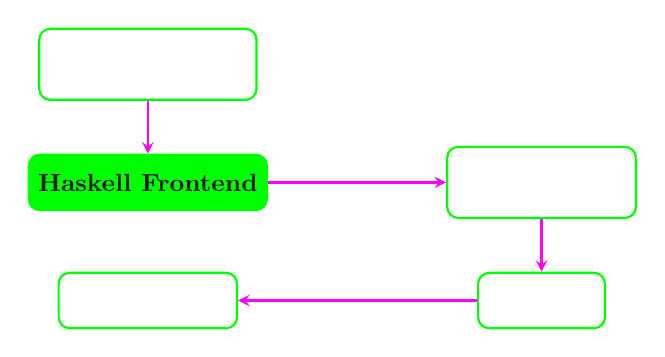
\begin{tikzpicture}[
        node distance=1.5cm,
        every node/.style={
            rectangle, 
            draw=fgdata, 
            thick, 
            text=white,
            align=center,
            rounded corners,
            minimum height=2em,
            font=\small
        },
        arrow/.style={
            ->, 
            >=stealth, 
            thick, 
            color=accent
        },
        highlight/.style={
            fill=fgdata,
            text=bgdata,
            font=\small\bfseries
        }
    ]
        \node (src) {Rust-alike Syntax\\FP Program};
        \node (front) [below of=src, highlight] {Haskell Frontend};
        \node (mlir) [right of=front, node distance=5cm] {MLIR Backend\\Optimization};
        \node (llvm) [below of=mlir] {LLVM IR};
        \node (bin) [left of=llvm, node distance=5cm] {Machine Code};

        \draw[arrow] (src) -- (front);
        \draw[arrow] (front) -- (mlir);
        \draw[arrow] (mlir) -- (llvm);
        \draw[arrow] (llvm) -- (bin);
    \end{tikzpicture}
\end{frame}

\begin{frame}{Frontend Pipeline}
    \centering
    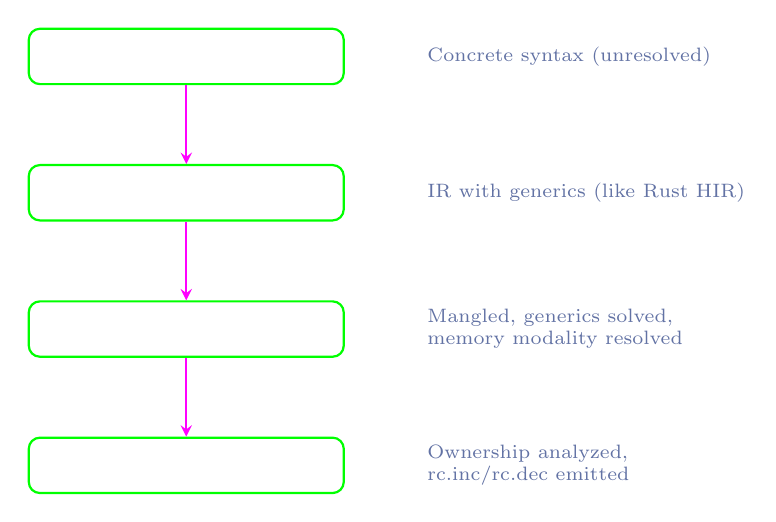
\begin{tikzpicture}[
        node distance=1.6cm,
        every node/.style={
            rectangle,
            draw=fgdata,
            thick,
            text=white,
            align=center,
            rounded corners,
            minimum height=2em,
            minimum width=4cm,
            font=\small
        },
        arrow/.style={
            ->,
            >=stealth,
            thick,
            color=accent
        },
        note/.style={
            draw=none,
            fill=none,
            text=comment,
            font=\scriptsize,
            minimum height=0pt,
            minimum width=0pt,
            inner sep=1pt,
            align=left
        }
    ]
        \node (pst) {Parser Syntax Tree};
        \node (semi) [below=1cm of pst] {Semi-Elaborated Syntax};
        \node (full) [below=1cm of semi] {Fully Elaborated Syntax};
        \node (mlir) [below=1cm of full] {MLIR};

        \draw[arrow] (pst) -- (semi);
        \draw[arrow] (semi) -- (full);
        \draw[arrow] (full) -- (mlir);

        % Annotations to the right
        \node[note, right=1cm of pst] {Concrete syntax (unresolved)};
        \node[note, right=1cm of semi] {IR with generics (like Rust HIR)};
        \node[note, right=1cm of full] {Mangled, generics solved,\\memory modality resolved};
        \node[note, right=1cm of mlir] {Ownership analyzed,\\rc.inc/rc.dec emitted};
    \end{tikzpicture}
\end{frame}

\begin{frame}{Why Two-Stage Elaboration?}
    Records in Reussir carry a \alert{memory modality} annotation:
    \begin{itemize}
        \item \texttt{[value]} --- copy semantics, no RC, stored inline.
        \item \texttt{[shared]} --- immutable, reference-counted (\texttt{Rc<T, Shared>}).
        \item \texttt{[regional]} --- mutable in region, reference-counted (\texttt{Rc<T, Flex/Rigid>}).
    \end{itemize}
    \vspace{0.3em}
    The modality determines \textbf{how memory operations are generated}.
    Value types need no RC ops; Shared/Regional types need
    \texttt{rc.inc}/\texttt{rc.dec} inserted by ownership analysis.

    \vspace{0.3em}
    $\Rightarrow$ We must \alert{fully resolve} modality and generics \textbf{before}
    ownership analysis can decide which operations to emit.
\end{frame}

\begin{frame}{Stage 1: Semi-Elaboration}
    \begin{itemize}
        \item Parse surface syntax into a \textbf{Semi-Elaborated IR}.
        \item Bidirectional type inference with \alert{unresolved generics}.
        \item Types carry \alert{flexivity} (\texttt{Irrelevant}, \texttt{Flex}, \texttt{Rigid}, \texttt{Regional}) --- not yet concrete memory decisions.
        \item Collect all generic instantiations across the program.
    \end{itemize}
    \vspace{0.5em}
    \textbf{Analogy}: Similar to Rust's HIR --- types are known but
    monomorphization has not happened yet.
\end{frame}

\begin{frame}{Stage 2: Full Elaboration}
    \begin{enumerate}
        \item \textbf{Monomorphize}: Instantiate all generic records and functions with concrete types.
        \item \textbf{Resolve modality}: Map flexivity to concrete capabilities:
        \begin{itemize}
            \item \texttt{[value]} $\to$ \texttt{TypeRecord} (bare, no RC wrapper)
            \item \texttt{[shared]} $\to$ \texttt{TypeRc(T, Shared)}
            \item \texttt{[regional] + [flex]} $\to$ \texttt{TypeRc(T, Flex)}
            \item \texttt{[regional] + [rigid]} $\to$ \texttt{TypeRc(T, Rigid)}
        \end{itemize}
        \item \textbf{Mangle names}: e.g.\ \texttt{Cell<u64>} $\to$ \texttt{\_RIC4CellyE}
    \end{enumerate}
    \vspace{0.5em}
    After this stage, every type is concrete --- ready for ownership analysis.
\end{frame}

\begin{frame}{PST $\to$ Semi: Bidirectional Type Checking}
    We use \alert{bidirectional type checking} to elaborate the parse tree:
    \begin{itemize}
        \item \textbf{Infer mode} ($\Gamma \vdash e \Rightarrow A$):
              Synthesize the type from the term.
              Used for literals, variables, projections, function calls.
        \item \textbf{Check mode} ($\Gamma \vdash e \Leftarrow A$):
              Verify the term against an expected type.
              Used for let bindings with annotations, return positions.
    \end{itemize}
    \vspace{0.3em}
    Generics remain as \alert{unresolved holes} ($?T$) during this stage ---
    each call site records which concrete types flow into generic parameters.
\end{frame}

\begin{frame}{Semi $\to$ Full: Flow-Based Generic Solver}
    Between semi and full elaboration, a \alert{flow-based generic solver}
    resolves all generic instantiations:
    \begin{itemize}
        \item Collect all type flows $\tau \leadsto ?T_i$ at call sites.
        \item Build a constraint graph and propagate concrete types.
        \item Produce a \textbf{GenericSolution}: $\text{GenericID} \to [\text{Type}]$.
    \end{itemize}
    \vspace{0.3em}
    Based on the algorithm from:
    \begin{quote}
        \small
        \textit{``Flow-Sensitive Type Inference for Scripting Languages''}\\
        OOPSLA 2025 \hfill {\color{comment}\texttt{doi:10.1145/3720472}}
    \end{quote}
    \vspace{0.2em}
    The solution drives monomorphization --- each unique instantiation
    produces a separate fully-elaborated function and record.
\end{frame}

\begin{frame}[fragile]{Demo: Value Modality}
    \begin{lstlisting}[basicstyle=\ttfamily\scriptsize\color{white}, language=]
struct [value] Matrix {
    m00: u64, m01: u64,
    m10: u64, m11: u64
}

fn matmul(a : Matrix, b : Matrix) -> Matrix {
    let m00 = a.m00 * b.m00 + a.m01 * b.m10;
    let m01 = a.m00 * b.m01 + a.m01 * b.m11;
    let m10 = a.m10 * b.m00 + a.m11 * b.m10;
    let m11 = a.m10 * b.m01 + a.m11 * b.m11;
    Matrix { m00: m00, m01: m01, m10: m10, m11: m11 }
}
    \end{lstlisting}
    \vspace{0.3em}
    \texttt{[value]} $\Rightarrow$ \textbf{No RC overhead}.
    \texttt{Matrix} is passed and returned by value (copy semantics).
\end{frame}

\begin{frame}[fragile]{Demo: Shared Modality}
    \begin{lstlisting}[basicstyle=\ttfamily\scriptsize\color{white}, language=]
struct [value] Box<T> { val : T }
struct [shared] RcBox<T> { val : T }

pub fn rc_project(rc : RcBox<u32>) -> u32 {
    rc.val
}

pub fn rc_project_chained(rc : RcBox<RcBox<u32>>) -> u32 {
    rc.val.val
}
    \end{lstlisting}
    \vspace{0.3em}
    \texttt{[shared]} $\Rightarrow$ \textbf{Immutable, reference-counted}.
    \texttt{RcBox<u32>} becomes \texttt{Rc<RcBox<u32>, Shared>} in Full IR.
    Projections borrow the inner value --- no copies needed.
\end{frame}

\begin{frame}[fragile]{Demo: Regional Mutation (\texttt{[field]})}
    \begin{lstlisting}[basicstyle=\ttfamily\scriptsize\color{white}, language=]
struct [regional] DLLink<T> {
    val: T,
    next: [field] DLLink<T>,
    prev: [field] DLLink<T>
}

regional fn push_back<T>(
    cursor : [flex] DLLink<T>, elem : T
) {
    let new_node = new(elem);
    new_node->prev := Nullable::NonNull{cursor};
    cursor->next := Nullable::NonNull{new_node};
}
    \end{lstlisting}
    \vspace{0.3em}
    \texttt{[field]} marks mutable fields within regional structs.
    The \texttt{->} operator enables in-place mutation on \texttt{[flex]} references.
\end{frame}

\begin{frame}{Ownership Analysis}
    After full elaboration, \textbf{Ownership Analysis} emits \texttt{rc.inc}/\texttt{rc.dec}:
    \begin{itemize}
        \item Each \alert{resource-relevant} (RR) parameter starts with ownership $= 1$.
        \item \textbf{Consuming uses} (function args, returns) transfer ownership.
        \item \textbf{Borrowing uses} (projections, match scrutinees) do not consume.
        \item \textbf{Early dec}: \texttt{rc.dec} placed at earliest point after last use.
        \item \textbf{Branch reconciliation}: All branches must reach same ownership state.
    \end{itemize}
    \vspace{0.3em}
\end{frame}

\section{Polymorphic FFI}

\begin{frame}{The FFI Challenge in FP Languages}
    RC-based runtime naturally embeds an \alert{ownership model}
    into the imperative world:
    \begin{itemize}
        \item \texttt{repr(C)} headers --- ABI-compatible RC layout.
        \item \texttt{Clone} $\leftrightarrow$ \texttt{rc.inc}, \texttt{Drop} $\leftrightarrow$ \texttt{rc.dec}.
        \item Rust code can hold and manipulate Reussir objects directly.
    \end{itemize}
    \vspace{0.3em}
    \textbf{Problem}: This only works for \alert{monomorphic} types.

    For \textbf{polymorphic} types (\texttt{Vec<T>}, \texttt{HashMap<K,V>}),
    Lean/Koka resort to \alert{boxed values} --- uniform representation
    with runtime type dispatch, losing type-specific layout and performance.
\end{frame}

\begin{frame}{Reussir's Approach: Monomorphic Instantiation}
    \textbf{Key insight}: Since Reussir already monomorphizes generics
    during full elaboration, we can do the same for FFI types.
    \vspace{0.3em}
    \begin{itemize}
        \item FFI libraries provide \alert{template} Rust source with
              \texttt{[:typename:]} placeholders.
        \item When generics are solved, substitute concrete types
              and compile each instantiation separately.
        \item No boxing --- \texttt{Vec<i64>} and \texttt{Vec<f64>}
              get their own specialized code, just like native Rust.
    \end{itemize}
    \vspace{0.3em}
    \textbf{Advantage}: Zero-overhead interop with Rust's type-specialized
    collections and data structures.
\end{frame}

\begin{frame}{RC Layout: Bridging Two Worlds}
    \centering
    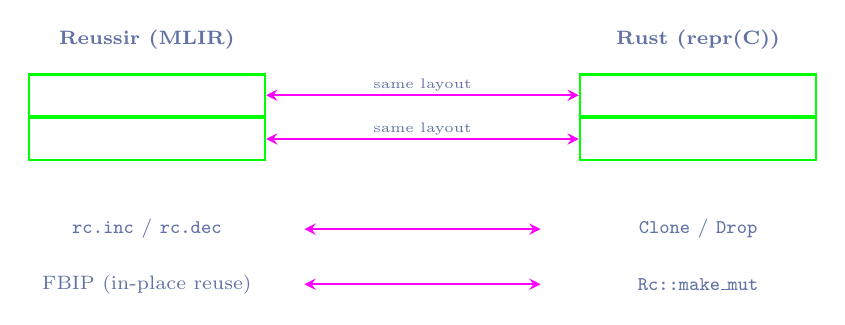
\begin{tikzpicture}[
        node distance=0.5cm,
        box/.style={
            rectangle,
            draw=fgdata,
            thick,
            text=white,
            align=center,
            font=\scriptsize,
            minimum width=3cm,
            minimum height=1.5em
        },
        label/.style={
            draw=none,
            fill=none,
            text=comment,
            font=\scriptsize,
            minimum height=0pt,
            inner sep=1pt,
            align=center
        },
        arrow/.style={
            <->,
            >=stealth,
            thick,
            color=accent
        }
    ]
        % Reussir side
        \node[label] (rl) at (-3.5, 2.2) {\textbf{Reussir (MLIR)}};
        \node[box] (rc) at (-3.5, 1.5) {\texttt{rc\_count}};
        \node[box, below=0pt of rc] (rd) {\texttt{data: T}};

        % Rust side
        \node[label] (rrl) at (3.5, 2.2) {\textbf{Rust (repr(C))}};
        \node[box] (rrc) at (3.5, 1.5) {\texttt{count: Cell<usize>}};
        \node[box, below=0pt of rrc] (rrd) {\texttt{data: UnsafeCell<T>}};

        % Arrows
        \draw[arrow] (rc.east) -- node[above, label, font=\tiny] {same layout} (rrc.west);
        \draw[arrow] (rd.east) -- node[above, label, font=\tiny] {same layout} (rrd.west);

        % Operations
        \node[label] at (-3.5, -0.2) {\texttt{rc.inc} / \texttt{rc.dec}};
        \node[label] at (3.5, -0.2) {\texttt{Clone} / \texttt{Drop}};
        \draw[arrow] (-1.5, -0.2) -- (1.5, -0.2);

        \node[label] at (-3.5, -0.9) {FBIP (in-place reuse)};
        \node[label] at (3.5, -0.9) {\texttt{Rc::make\_mut}};
        \draw[arrow] (-1.5, -0.9) -- (1.5, -0.9);
    \end{tikzpicture}
    \vspace{0.3em}

    \texttt{repr(C)} ensures identical memory layout.
    Rust's \texttt{make\_mut} is the same idea as FBIP: mutate in-place
    when uniquely owned, copy otherwise.
\end{frame}

\begin{frame}[fragile]{Polymorphic FFI: Template Mechanism}
    \begin{lstlisting}[basicstyle=\ttfamily\scriptsize\color{white}, language=]
// MLIR: Before compilation
reussir.polyffi
    texture("
        extern crate reussir_rt; // shipped as HIR Rlib
        use reussir_rt::collections::vec::Vec;

        pub unsafe extern "C"
        fn vec_new() -> Vec<[:typename:]> {
            Vec::new()
        }

        pub unsafe extern "C"
        fn vec_push(v: Vec<[:typename:]>,
                    e: [:typename:])
            -> Vec<[:typename:]> {
            v.push(e)
        }
    ")
    substitutions({"typename" = "f64"})
    \end{lstlisting}
\end{frame}

\begin{frame}[fragile]{Polymorphic FFI: After Compilation}
    \begin{lstlisting}[basicstyle=\ttfamily\scriptsize\color{white}, language=]
// Opaque FFI type with cleanup hook
!Vecf64 = !reussir.rc<!reussir.ffi_object<
    "::reussir_rt::collections::vec::Vec<f64>",
    @__polyffi_Vec_f64_drop
>>

// MLIR: After CompilePolymorphicFFI pass
reussir.polyffi
    compiled(dense_resource<blob> : tensor<...xi8>)
    // ^ Embedded LLVM bitcode from rustc

// Generated declarations are available
func.func private @vec_f64_new() -> !Vecf64
func.func private @vec_f64_push(
    !Vecf64, f64) -> !Vecf64
    \end{lstlisting}
\end{frame}

\begin{frame}{Compilation Pipeline for FFI}
    \centering
    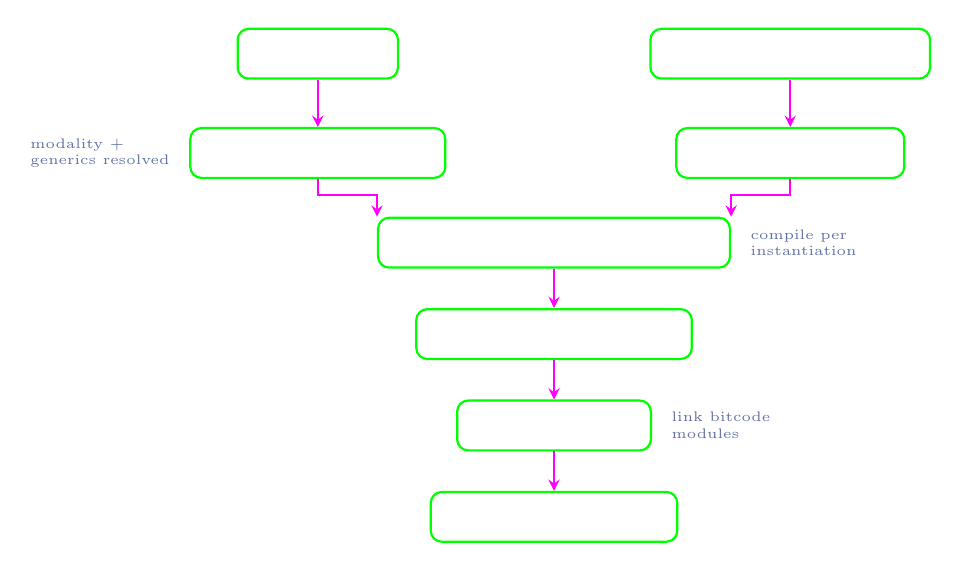
\begin{tikzpicture}[
        every node/.style={
            rectangle,
            draw=fgdata,
            thick,
            text=white,
            align=center,
            rounded corners,
            minimum height=1.8em,
            font=\scriptsize
        },
        arrow/.style={
            ->,
            >=stealth,
            thick,
            color=accent
        },
        note/.style={
            draw=none,
            fill=none,
            text=comment,
            font=\tiny,
            minimum height=0pt,
            minimum width=0pt,
            inner sep=1pt,
            align=left
        }
    ]
        % Left: Reussir path
        \node (rr) at (-3, 0) {Reussir Source};
        \node (full) [below=0.6cm of rr] {Full IR (generics solved)};

        % Right: Rust path
        \node (rs) at (3, 0) {Rust FFI Templates (HIR)};
        \node (rshir) [below=0.6cm of rs] {\texttt{[:typename:]} markers};

        % Merge point
        \node (mono) at (0, -2.4) {Monomorphize + \texttt{rustc} $\to$ bitcode};

        % Bottom row
        \node (mlir) [below=0.5cm of mono] {MLIR (embedded bitcode)};
        \node (llvm) [below=0.5cm of mlir] {LLVM IR (linked)};
        \node (bin) [below=0.5cm of llvm] {Binary + \texttt{libreussir\_rt}};

        \draw[arrow] (rr) -- (full);
        \draw[arrow] (rs) -- (rshir);
        \draw[arrow] (full.south) -- ++(0, -0.2) -| (mono.north west);
        \draw[arrow] (rshir.south) -- ++(0, -0.2) -| (mono.north east);
        \draw[arrow] (mono) -- (mlir);
        \draw[arrow] (mlir) -- (llvm);
        \draw[arrow] (llvm) -- (bin);

        % Annotations
        \node[note, left=0.2cm of full] {modality +\\generics resolved};
        \node[note, right=0.2cm of mono] {compile per\\instantiation};
        \node[note, right=0.2cm of llvm] {link bitcode\\modules};
    \end{tikzpicture}
\end{frame}

\begin{frame}{Boxed vs Monomorphic: Comparison}
    \centering
    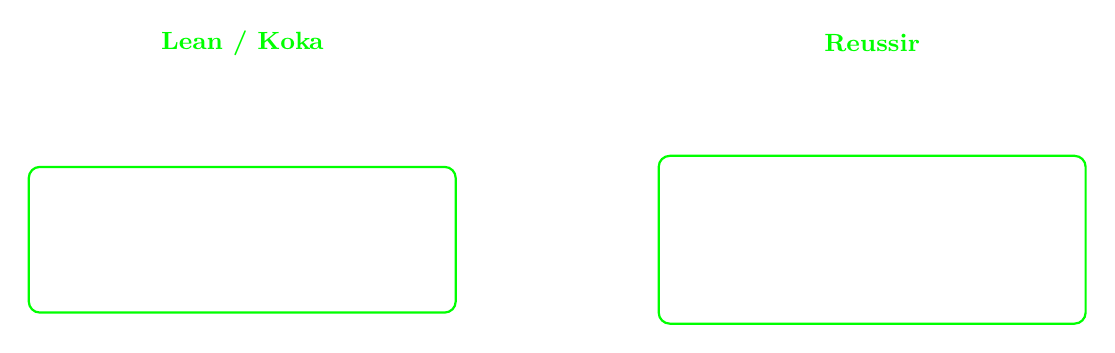
\begin{tikzpicture}[
        box/.style={
            rectangle,
            draw=fgdata,
            thick,
            text=white,
            align=left,
            rounded corners,
            font=\scriptsize,
            inner sep=6pt
        },
        label/.style={
            draw=none,
            fill=none,
            text=fgdata,
            font=\small\bfseries,
            inner sep=1pt
        }
    ]
        % Lean/Koka
        \node[label] at (-4, 3.5) {Lean / Koka};
        \node[box, text width=5cm] at (-4, 1) {
            \texttt{Vec<T>} $\to$ \texttt{Array Object}\\[3pt]
            \textbullet\ Uniform boxed representation\\
            \textbullet\ Runtime type dispatch\\
            \textbullet\ Extra indirection for primitives\\
            \textbullet\ Cannot inline type-specific ops
        };

        % Reussir
        \node[label] at (4, 3.5) {Reussir};
        \node[box, text width=5cm] at (4, 1) {
            \texttt{Vec<T>} $\to$ \texttt{Vec<f64>}, \texttt{Vec<i64>}, \dots\\[3pt]
            \textbullet\ Type-specialized code per instantiation\\
            \textbullet\ No boxing overhead\\
            \textbullet\ Native Rust \texttt{Vec} layout\\
            \textbullet\ Full LLVM optimization across FFI
        };
    \end{tikzpicture}
\end{frame}

\section*{}

\begin{frame}
    \centering
    \vspace{2cm}
    {\Huge\color{fgdata} Thank you!}
    \vspace{1.5cm}

    {\large\color{white} Reussir}\\[0.3em]
    {\color{comment} A Memory Reuse IR Playground for FP Languages}
\end{frame}

\end{document}
